\chapter{Introduction}

%\begin{itemize}
%    \item What is \texttt{IPPL}.
%    \item Where does FEM come into play.
%    \item FEM currently only supports Lagrange Elements.
%    \item Would like to solve problems from Electromagnetism \( \implies \) Need Nédélec.
%    \item Quickly explain what Nédélec is.
%    \item To this extent implement the Nédélec finite element space in \texttt{IPPL}.
%\end{itemize}

%\begin{figure}[!th]
%    \centering
%    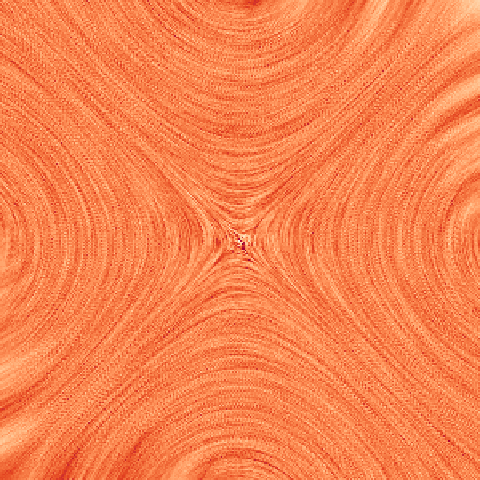
\includegraphics[width=0.5\textwidth]{figures/introduction/hero.png}
%    \caption{Function obtained with the Nédélec FEM framework.}
%    \label{fig:exampleNedlec}
%\end{figure}

\texttt{IPPL} \cite{muralikrishnan2024scaling} stands for Independent Parallel Particle layer and is a performance portable C++ library designed for Particle-Mesh methods. One primary part of \texttt{IPPL} is a Particle In Cell (PIC) loop, in which particles are simulated in a Lagrangian frame, while simultaneously certain properties are calculated in an Eulerian frame (on the mesh), and then these properties are used to update the particles. So we have two independent building blocks, one is the simulation of particles, while the other one is the solving of PDEs in the Eulerian frame. One method that can be used to solve the PDEs and which already is part of \texttt{IPPL} is the Finite Element Method (FEM). For a general introduction into FEM please refer to \cite{femBook} and for an explanation on how FEM is implemented in \texttt{IPPL} please refer to \cite{femIppl}.\medskip

Currently the FEM framework in \texttt{IPPL} only supports first order Lagrange basis functions, which limits the range of solvable PDEs to scalar functions. In the future we would like to be able to solve problems from electromagnetism, therefore we need to define a new finite element space which supports such vector fields. A natural choice for the electric field in the case of electromagnetism are the Nédélec basis functions \cite{nedelec}, in order to also have the magnetic one a different finite element space would have to be used, namely Raviart-Thomas. The Nédélec basis functions create a \(H(\text{curl}, \Omega)\)-conforming finite element space, where the basis functions are vector fields defined on the edges of the mesh and they exist for 2D and 3D. In the rest of this report we will look into the implementation of the Nédélec space in \texttt{IPPL} and some numerical results in order to test the correctness of the implementation and to provide performance characteristics. 